\documentclass[tikz, border=3.14mm]{standalone}
\usepackage{pgfplots}
\pgfplotsset{compat=1.18}
\usepgfplotslibrary{groupplots}

\begin{document}
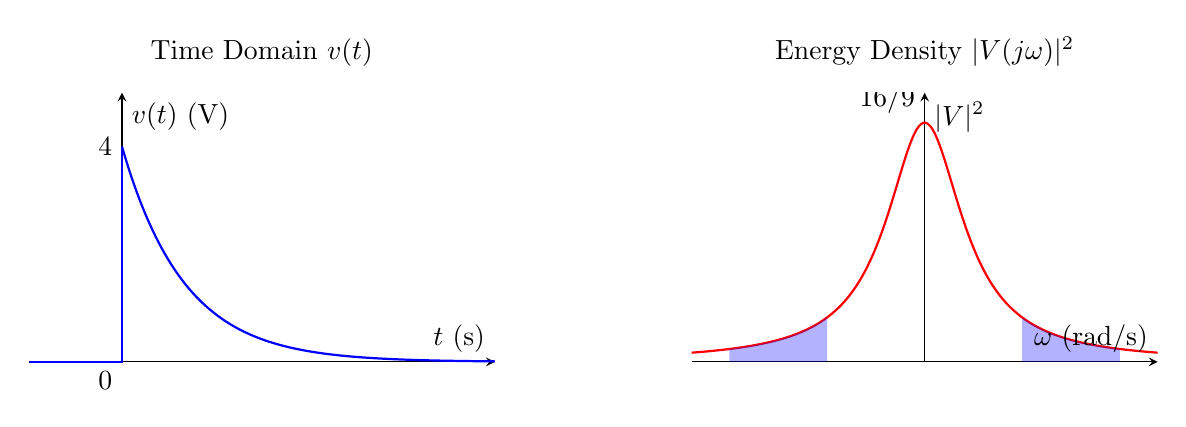
\begin{tikzpicture}
    \begin{groupplot}[
        group style={group size=2 by 1, horizontal sep=2.5cm},
        axis lines = middle,
        width = 7.5cm, height = 5cm,
        xtick = \empty, ytick = \empty
    ]
        % Time Domain: 4e^{-3t}u(t)
        \nextgroupplot[
            title = {Time Domain $v(t)$},
            xlabel = {$t$ (s)},
            ylabel = {$v(t)$ (V)},
            xmin = -0.5, xmax = 2,
            ymin = 0, ymax = 5,
            clip = false
        ]
        \addplot[thick, blue, domain=0:2, samples=100] {4*exp(-3*x)};
        \draw[thick, blue] (axis cs:-0.5, 0) -- (axis cs:0, 0) -- (axis cs:0, 4);
        \node[anchor=east] at (axis cs:0, 4) {4};
        \node[anchor=north east] at (axis cs:0, 0) {0};

        % Frequency Domain: |V(jw)|^2 = 16 / (9 + w^2)
        % w range: 1 Hz -> 2*pi approx 6.28, 2 Hz -> 4*pi approx 12.57
        \nextgroupplot[
            title = {Energy Density $|V(j\omega)|^2$},
            xlabel = {$\omega$ (rad/s)},
            ylabel = {$|V|^2$},
            xmin = -15, xmax = 15,
            ymin = 0, ymax = 2,
            samples = 200
        ]
        \addplot[thick, red, domain=-15:15] {16/(9 + x^2)};
        
        % Passband Shading (1 < |f| < 2 Hz => 2pi < |w| < 4pi)
        \addplot[fill=blue, fill opacity=0.3, draw=none, domain=6.28:12.57] {16/(9 + x^2)} \closedcycle;
        \addplot[fill=blue, fill opacity=0.3, draw=none, domain=-12.57:-6.28] {16/(9 + x^2)} \closedcycle;
        
        \draw[<->, blue, thick] (axis cs:6.28, -0.15) -- node[below, pos=0.5, font=\tiny] {Passband} (axis cs:12.57, -0.15);
        \node[anchor=north, font=\tiny] at (axis cs:6.28, 0) {$2\pi$};
        \node[anchor=north, font=\tiny] at (axis cs:12.57, 0) {$4\pi$};
        \node[anchor=south east] at (axis cs:0, 1.77) {$16/9$};

    \end{groupplot}
\end{tikzpicture}
\end{document}
